\phantomsection\numberedsection{RF8 Gestión de Exportación}

\subsection*{Descripción}
El sistema permite a los usuarios exportar productos seleccionados desde Mini PIM a Amazon, configurando atributos obligatorios y opcionales de forma personalizable.

\vspace{0.15cm}

\textbf{Pre-condición}\par
El usuario ha iniciado sesión en su cuenta en Mini PIM y existen productos en el sistema con los atributos obligatorios necesarios.

\vspace{0.15cm}

\textbf{Post-condición}
\begin{itemize}
    \item Caso de éxito: Los productos seleccionados son exportados exitosamente al formato CSV requerido por Amazon y están listos para su carga.
    \item Caso mínimo: El sistema notifica al usuario cualquier error o dato faltante, permitiendo realizar las correcciones necesarias.
\end{itemize}

\textbf{Prioridad:}
Alta

\vspace{0.15cm}

\textbf{Autores:}
Diego Sicre, Angel Escaño y Francisco Javier Jordá Garay.

\vspace{0.15cm}

\textbf{Control de cambios: } Versión 1: Definición del caso de uso

\numberedsubsection{Escenario principal}
\begin{enumerate}
    \item El usuario accede a la sección \enquote{Productos}.
    \item El sistema muestra un listado de productos con los siguientes atributos:
    \begin{itemize}
        \item Thumbnail
        \item SKU
        \item Nombre
        \item Hasta cinco atributos de usuario.
    \end{itemize}
    \item El usuario puede activar o desactivar filtros mediante toggles:\footnote{No necesariamente se tienen que seleccionar ambas opciones de filtrado para encontrar un producto. Aquí exponemos las dos alternativas combinables que tiene el usuario para filtrar. Por defecto ambos están desactivados.}
    \begin{itemize}
        \item Filtro por categoría: El usuario activa el toggle correspondiente y selecciona una categoría del \emph{ComboBox}.
        \item Filtro por fecha: El usuario activa el toggle correspondiente y selecciona un día en el \emph{Calendario}.
    \end{itemize}
    \item El usuario puede usar el botón \enquote{Clear} para desactivar todos los filtros antes de realizar un nuevo filtro.
    \item Según los filtros activos, el sistema actualiza la lista de productos mostrados.
    \item El usuario selecciona uno o más productos para exportar.
    \item El usuario hace clic en el botón \enquote{CSV}.
    \item El sistema muestra un formulario para configurar el mapeo de atributos obligatorios, incluyendo:
    \begin{itemize}
        \item SKU: Se utiliza el SKU del producto en el sistema.
        \item Título: Se selecciona el \textit{Label} del producto.
        \item Fulfilled by: Nombre de la cuenta.
        \item Amazon\_SKU: Permite elegir entre SKU/GTIN.
        \item Precio: Selección de un atributo de usuario como precio del producto.
        \item Offer Price: Configuración general como \texttt{TRUE/FALSE/RANDOM}.
    \end{itemize}
    \item El sistema verifica la validez de los atributos obligatorios seleccionados.
    \item El usuario confirma la configuración de mapeo obligatorio y selecciona \enquote{Continue}.
    \item El sistema permite seleccionar atributos adicionales de usuario\footnote{Se tomaron en cuenta las consideraciones descritas en \href{https://buywithprime.amazon.com/knowledge-center/csv-import?utm_medium=website\&utm_source=direct\#standalone-product}{CSV Import} de Amazon para manejar la elección de atributos adicionales de usuario correctamente.} para exportar.
    \item El usuario selecciona \enquote{Confirmar} para finalizar la exportación.
    \item El sistema genera un archivo CSV.
\end{enumerate}

\numberedsubsection{Escenarios alternativos}
\begin{description}
    \item[3.a] El usuario no encuentra el producto al filtrar por categoría.
    \begin{enumerate}
        \item[3.a.1] El sistema muestra un mensaje indicando que no existen productos con esa categoría.
    \end{enumerate}
    \item[3.b] El usuario no encuentra el producto al filtrar por fecha.
    \begin{enumerate}
        \item[3.b.1] El sistema muestra un mensaje indicando que no hay productos disponibles en el rango seleccionado.
    \end{enumerate}
    \item[3.c] El usuario no activa ningún toggle de filtro.
    \begin{enumerate}
        \item[3.c.1] El sistema muestra todos los productos disponibles en la lista.
    \end{enumerate}
    \item[4.a] El usuario utiliza el botón \enquote{Clear} para desactivar todos los filtros.
    \begin{enumerate}
        \item[4.a.1] El sistema desactiva el filtro por fecha y por categoría actualizan la lista mostrando todos los productos disponibles en la lista.
    \end{enumerate}
    \item[7.a] No hay productos seleccionados.
    \begin{enumerate}
        \item[7.a.1] El sistema notifica al usuario que debe seleccionar al menos un producto para exportar.
    \end{enumerate}
    \item[9.a] No existe ningún atributo de usuario de tipo \texttt{float} o \texttt{entero} para \enquote{Precio}.
    \begin{enumerate}
        \item[9.a.1] El sistema muestra un mensaje de error indicando que no se puede proceder con la exportación, ya que no es posible mapear un precio.
    \end{enumerate}
    \item[10.a] Falta algún atributo obligatorio.
    \begin{enumerate}
        \item[10.a.1] El sistema notifica al usuario de que faltan atributos obligatorios.
    \end{enumerate}
\end{description}

\numberedsubsection{Casos de Prueba}

\underline{Escenario: Alternativo 3.a (no se encuentran productos al filtrar por categoría)}\par
\vspace{0.15cm}
\textbf{Dado} que el usuario ha iniciado sesión con su cuenta de usuario correspondiente,\par
\textbf{Y} se encuentra en el apartado de \enquote{Productos},\par
\textbf{Y} filtra productos por una categoría específica,\par
\textbf{Y} no hay productos asociados a esa categoría,\par
\textbf{Cuando} el sistema no encuentra productos con la categoría seleccionada,\par
\textbf{Entonces} el sistema muestra un mensaje indicando que no existen productos con esa categoría.\par

\vspace{0.20cm}

\underline{Escenario: Alternativo 3.b (no se encuentran productos al filtrar por fecha)}\par
\vspace{0.15cm}
\textbf{Dado} que el usuario ha iniciado sesión con su cuenta de usuario correspondiente,\par
\textbf{Y} se encuentra en el apartado de \enquote{Productos},\par
\textbf{Y} filtra productos por fecha seleccionando un rango en el calendario,\par
\textbf{Y} no hay productos con modificaciones en el rango especificado,\par
\textbf{Cuando} el sistema no encuentra productos dentro del rango de fechas seleccionado,\par
\textbf{Entonces} el sistema muestra un mensaje indicando que no hay productos disponibles en ese rango de fechas.\par

\vspace{0.20cm}

\underline{Escenario: Alternativo 3.c (ningún toggle de filtro activo)}\par
\vspace{0.15cm}
\textbf{Dado} que el usuario ha iniciado sesión con su cuenta de usuario correspondiente,\par
\textbf{Y} se encuentra en el apartado de \enquote{Productos},\par
\textbf{Cuando} el usuario no activa ningún filtro (ni por categoría ni por fecha),\par
\textbf{Entonces} el sistema muestra todos los productos disponibles en la lista, sin aplicar ningún filtro.\par

\vspace{0.20cm}

\underline{Escenario: Alternativo 4.a (desactivar todos los filtros)}\par
\vspace{0.15cm}
\textbf{Dado} que el usuario ha iniciado sesión con su cuenta de usuario correspondiente,\par
\textbf{Y} se encuentra en el apartado de \enquote{Productos},\par
\textbf{Y} tiene filtros activados por categoría y/o fecha,\par
\textbf{Cuando} el usuario hace clic en el botón \enquote{Clear},\par
\textbf{Entonces} el sistema desactiva los filtros por fecha y por categoría,\par
\textbf{Y} actualiza la lista mostrando todos los productos disponibles en la lista sin ningún filtro aplicado.\par

\vspace{0.20cm}
\newpage
\underline{Escenario: Alternativo 7.a (no hay productos seleccionados)}\par
\vspace{0.15cm}
\textbf{Dado} que el usuario ha iniciado sesión con su cuenta de usuario correspondiente,\par
\textbf{Y} se encuentra en el apartado de \enquote{Productos},\par
\textbf{Y} no ha seleccionado ningún producto de la lista,\par
\textbf{Cuando} hace clic en el botón \enquote{CSV} para exportar,\par
\textbf{Entonces} el sistema muestra un mensaje indicando que debe seleccionar al menos un producto para la exportación.\par

\vspace{0.20cm}

\underline{Escenario: Alternativo 9.a (No existe ningún atributo de tipo \texttt{float} o \texttt{entero})}\par\vspace{0.15cm}
\vspace{0.15cm}
\textbf{Dado} que el usuario ha iniciado sesión con su cuenta de usuario correspondiente,\par
\textbf{Y} se encuentra en el apartado de \enquote{Productos},\par
\textbf{Y} selecciona productos de la lista,\par
\textbf{Y} hace clic en el botón \enquote{CSV},\par
\textbf{Y} configura el atributo correspondiente a \enquote{Precio},\par
\textbf{E} intenta continuar seleccionando \enquote{Continue},\par
\textbf{Cuando} el sistema detecta que el atributo de usuario seleccionado para \enquote{Precio} no es de tipo \texttt{float} o \texttt{entero},\par
\textbf{Entonces} muestra un mensaje de error indicando que no se puede proceder con la exportación, ya que no es posible mapear un precio.\par

\vspace{0.20cm}

\underline{Escenario: Alternativo 10.a (Falta algún atributo obligatorio)}\par
\vspace{0.15cm}
\textbf{Dado} que el usuario ha iniciado sesión con su cuenta de usuario correspondiente,\par
\textbf{Y} se encuentra en el apartado de \enquote{Productos},\par
\textbf{Y} selecciona productos de la lista,\par
\textbf{Y} hace clic en el botón \enquote{CSV},\par
\textbf{Y} está configurando el mapeo de atributos obligatorios,\par
\textbf{Cuando} intenta continuar seleccionando \enquote{Continue} con uno o más atributos obligatorios faltantes,\par
\textbf{Entonces} el sistema notifica al usuario que faltan atributos obligatorios,\par
\textbf{Y} permite al usuario corregirlos antes de continuar con la exportación.\par


\numberedsubsection{Bocetos}
\begin{figure}[H]
    \includegraphics[width=1\linewidth]{assets/mockups/RF8 filtrado y selección de productos.png}
    \caption{Pantalla principal de exportación en apartado \enquote{Productos} filtrado por fecha y categoría}
\end{figure}

\begin{figure}[H]
    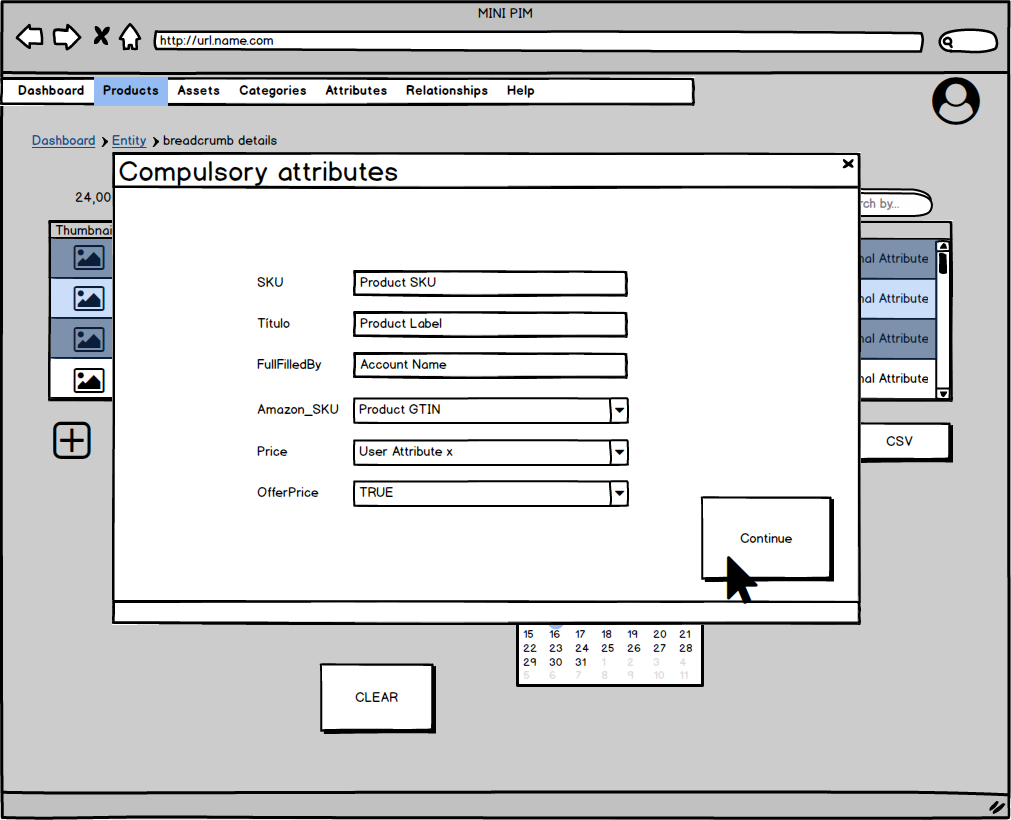
\includegraphics[width=1\linewidth]{assets/mockups/RF8 Seleccion de atributos obligatorios.png}
    \caption{Formulario de configuración de mapeo de atributos obligatorios tras clicar \enquote{CSV}}
\end{figure}

\begin{figure}[H]
    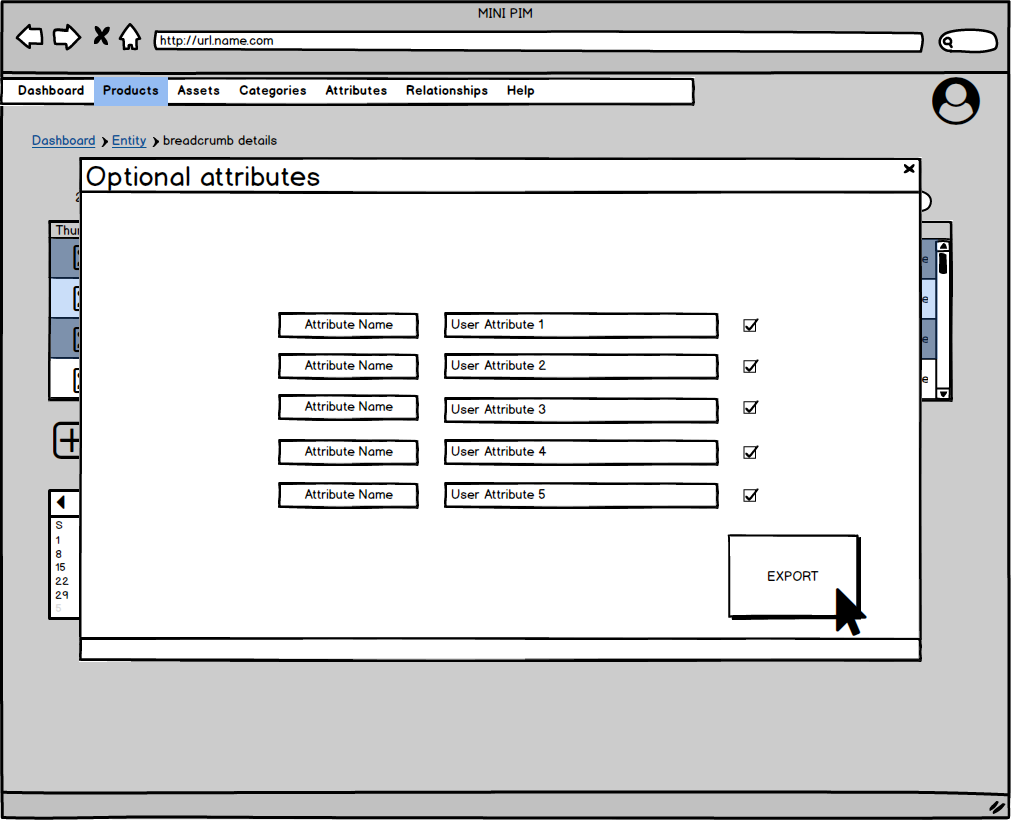
\includegraphics[width=1\linewidth]{assets/mockups/RF8 Seleccion atributos opcionales.png}
    \caption{Selección de atributos de usuario opcionales en la exportación}
\end{figure}

\begin{figure}[H]
    \includegraphics[width=1\linewidth]{assets/mockups/RF8 selección de productos (sin filtros).png}
    \caption{Caso donde no hay ningún filtro activado}
\end{figure}

\numberedsubsection{Diagrama de Secuencia}
\begin{figure}[H]
    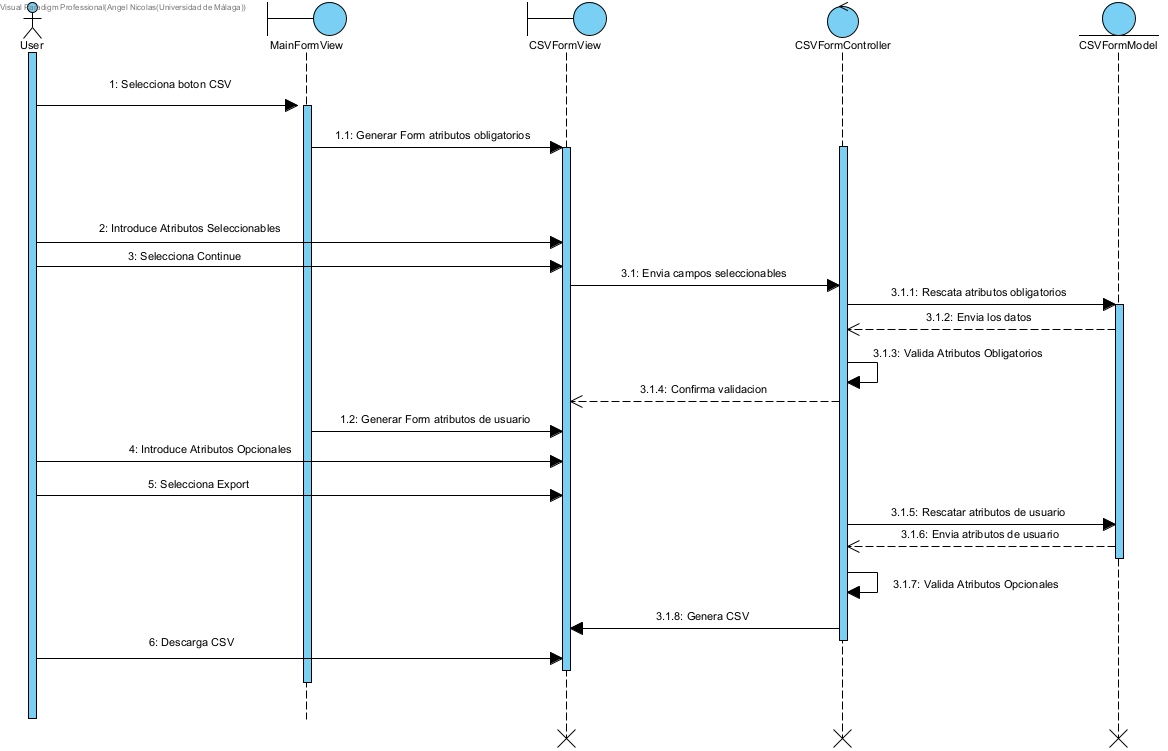
\includegraphics[width=1\linewidth]{assets/sequence/RF8.jpg}
    \caption{Diagrama de Secuencia para la gestión de exportación}
\end{figure}